\documentclass[12pt,a4paper]{article}
\usepackage[UTF8]{ctex}
\usepackage{geometry}
\geometry{left=2.5cm,right=2.5cm,top=2.5cm,bottom=2.5cm}
\usepackage{graphicx}
\usepackage{amsmath,amssymb}
\usepackage{listings}
\usepackage{xcolor}
\usepackage{float}
\usepackage{caption}
\usepackage{booktabs}
\usepackage{multirow}
\usepackage{array}
\usepackage{hyperref}

\hypersetup{
    colorlinks=true,
    linkcolor=blue!60!black,
    citecolor=blue!60!black,
    urlcolor=teal!70!black,
}

\lstset{
    language=Python,
    basicstyle=\ttfamily\small,
    keywordstyle=\color{blue},
    commentstyle=\color{gray},
    stringstyle=\color{red},
    numbers=left,
    numberstyle=\tiny\color{gray},
    frame=single,
    breaklines=true,
    showstringspaces=false,
    tabsize=4
}

% ----- 实验数字（H20 / batch=8 / 1024 点）-----
\newcommand{\PNparams}{3.47}      % M
\newcommand{\PNNparams}{1.48}     % M
\newcommand{\PNoa}{87.80}         % single-vote OA  (%)
\newcommand{\PNoaVote}{87.97}     % 12-vote OA      (%)
\newcommand{\PNmacc}{84.86}       % single-vote mAcc(%)
\newcommand{\PNmaccVote}{85.10}   % 12-vote mAcc    (%)
\newcommand{\PNbestEp}{164}       % best epoch
\newcommand{\PNNoa}{91.13}        % single-vote OA  (%)
\newcommand{\PNNoaVote}{91.77}    % 12-vote OA      (%)
\newcommand{\PNNmacc}{89.01}      % single-vote mAcc(%)
\newcommand{\PNNmaccVote}{88.98}  % 12-vote mAcc    (%)
\newcommand{\PNNbestEp}{112}      % best epoch
\newcommand{\PNlatency}{0.167}    % ms/sample
\newcommand{\PNNlatency}{4.07}    % ms/sample
\newcommand{\PNspeed}{5994}       % samples/sec
\newcommand{\PNNspeed}{245}       % samples/sec
\newcommand{\speedRatio}{24.4}    % PointNet 比 PointNet++ 快多少倍
\newcommand{\PNpaperOa}{89.2}     % 论文 PointNet OA
\newcommand{\PNNpaperOa}{91.9}    % 论文 PointNet++ SSG with normal OA

\title{\textbf{几何计算前沿\quad 第三次作业} \\ ModelNet40 三维形状分类：PointNet 与 PointNet++ 复现与对比}
\author{刘智琦 2300012860}
\date{\today}

\begin{document}
\maketitle

\begin{abstract}
本次作业基于 PyTorch 从零实现了两种经典点云分类方法 \textbf{PointNet}~\cite{qi2017pointnet} 与 \textbf{PointNet++ SSG}~\cite{qi2017pointnetpp}，并在 ModelNet40~\cite{wu20153d} 数据集上完成训练与评估。本报告介绍两个方法的核心思想、给出实现细节与训练曲线、对比单次与多次投票评估精度，并从参数量、推理速度、分类效果三个维度做横向分析。完整代码与训练好的权重见同目录 \texttt{src/} 与 \texttt{checkpoints/}。
\end{abstract}

\section{任务与数据集}

\subsection{任务定义}
给定一个表示三维物体的点云 $\mathcal{P}=\{p_i\}_{i=1}^{N},\ p_i\in\mathbb{R}^3$（可附带法向量等额外通道），输出该物体属于 40 类常见类别中的哪一类。这是 3D 视觉与几何深度学习的"helloworld"基准，要求模型对点的\textbf{排列不变性}（permutation invariance）以及\textbf{刚性变换}（rotation, translation, scaling）的鲁棒性。

\subsection{ModelNet40}
ModelNet40 由普林斯顿团队于 2015 年提出，包含 40 类 CAD 模型共 12{,}311 个三维网格（OFF 格式），按官方划分：训练集 9{,}843 个、测试集 2{,}468 个。本工作把每个 mesh 离线均匀采样 10{,}000 个表面点（含法向量），训练时再随机抽取 1{,}024 点送入网络。点云在喂入网络前做\textbf{中心化与单位球归一化}：
\begin{equation}
\tilde{p}_i = \frac{p_i - \bar{p}}{\max_j \|p_j - \bar{p}\|}.
\end{equation}

\subsection{数据增广}
训练时对每个样本独立施加：绕 $z$ 轴随机旋转 $\theta\sim\mathcal{U}(0,2\pi)$、各向同性缩放 $s\sim\mathcal{U}(0.8,1.25)$、随机平移 $t\sim\mathcal{U}([-0.1,0.1]^3)$、以及高斯抖动 $\delta\sim\mathcal{N}(0,0.01^2)$（截断到 $\pm 0.05$）。法向量同步旋转以保持几何一致性。

\section{方法}

\subsection{PointNet (CVPR 2017)}
PointNet 的核心洞察是：在点的\textbf{排列不变性}约束下，最一般的形式是先把每个点独立映射到高维特征空间，再通过一个\textbf{对称聚合函数}（如 max pool）合成全局特征。论文采用了一个非常简洁的结构：
\begin{equation}
f(\mathcal{P}) = \gamma\Big(\,\underset{i=1,\dots,N}{\max}\, h(p_i)\Big),
\end{equation}
其中 $h:\mathbb{R}^3\!\to\!\mathbb{R}^{1024}$ 是逐点共享 MLP，$\gamma$ 是一个 FC 分类头。论文证明了在 $\max$ 聚合下网络是排列不变的"通用近似器"。为了对刚性变换鲁棒，PointNet 在输入与中间特征上各插入一个 \textbf{T-Net} 学习刚性对齐矩阵：
\begin{equation}
T_{\text{input}}\in\mathbb{R}^{3\times 3},\quad T_{\text{feat}}\in\mathbb{R}^{64\times 64}.
\end{equation}
训练时对 $T_{\text{feat}}$ 加正交正则 $\|T T^\top - I\|_F^2$ 以避免特征空间过度形变。本实现完全遵循上述结构（见 \texttt{src/pointnet/model.py}），参数量 \PNparams\,M。

\subsection{PointNet++ SSG (NeurIPS 2017)}
PointNet 的明显短板是\textbf{缺乏局部结构归纳偏置}——所有点都共享同一套全局特征。PointNet++ 借鉴 CNN 的层级感受野思想，提出 \textbf{Set Abstraction (SA)} 模块：
\begin{enumerate}
    \item \textbf{Sampling}：用 Farthest Point Sampling (FPS) 从输入点集中均匀采样 $S$ 个中心点；
    \item \textbf{Grouping}：对每个中心点用 ball query（半径 $r$）搜集邻域内最多 $K$ 个点；
    \item \textbf{Pointnet}：把每个邻域当作一个小点集喂给共享 MLP + max pool，得到该中心点的局部特征。
\end{enumerate}
SSG (Single-Scale Grouping) 版本逐层降采样并扩大感受野：
\begin{center}
\begin{tabular}{lcccc}
\toprule
层 & 中心点 $S$ & 半径 $r$ & 邻域 $K$ & MLP 输出维度 \\
\midrule
SA1 & 512  & 0.2 & 32 & $[64,64,128]$ \\
SA2 & 128  & 0.4 & 64 & $[128,128,256]$ \\
SA3 (global) & 1 & — & 全部 & $[256,512,1024]$ \\
\bottomrule
\end{tabular}
\end{center}
最后接一个 FC 分类头。本实现使用 \textbf{xyz + 三维法向量} 作为输入（共 6 通道，与原作者推荐配置一致）。参数量 \PNNparams\,M。

\paragraph{纯 PyTorch 实现 FPS / Ball Query / Group。}
原始 PointNet++ 仓库为 FPS、Ball Query、Grouping 提供了 CUDA C++ 扩展以加速。考虑到本课程作业的可移植性、以及 CUDA 13.0 工具链与上游扩展存在 ABI 兼容性问题，本实现使用 \textbf{纯 PyTorch}（\texttt{torch.cdist} + \texttt{topk} + 高级索引）实现这三个 op（见 \texttt{src/pointnet2/ops.py}）。代价是单 epoch 时间约为 CUDA 版的 3\textendash 5 倍，但 H20 算力盈余足以容纳。

\section{实验设置}

\paragraph{硬件。} 单卡 NVIDIA H20（97\,GB 显存），CUDA 13.0，PyTorch 2.11.

\paragraph{超参数。}
\begin{itemize}
    \item 优化器：Adam，初始学习率 $10^{-3}$，权重衰减 $10^{-4}$；
    \item 调度：StepLR，每 20 个 epoch 学习率衰减为 0.7；
    \item Batch size $=32$，训练 250 个 epoch；
    \item PointNet 加 $10^{-3}$ 强度的 feature transform 正则；
    \item 训练点数 $N=1024$，PointNet 仅用 xyz，PointNet++ 同时用 xyz 与法向量；
    \item 评估：在 \texttt{test} 集上记录 OA (Overall Accuracy) 与 mAcc (Class-balanced Mean Accuracy)；可选 12 次随机采样投票（与原 PointNet 论文一致）。
\end{itemize}

\section{结果}

\subsection{训练曲线}
训练损失与测试 OA 曲线见图~\ref{fig:curves}。

\begin{figure}[H]
    \centering
    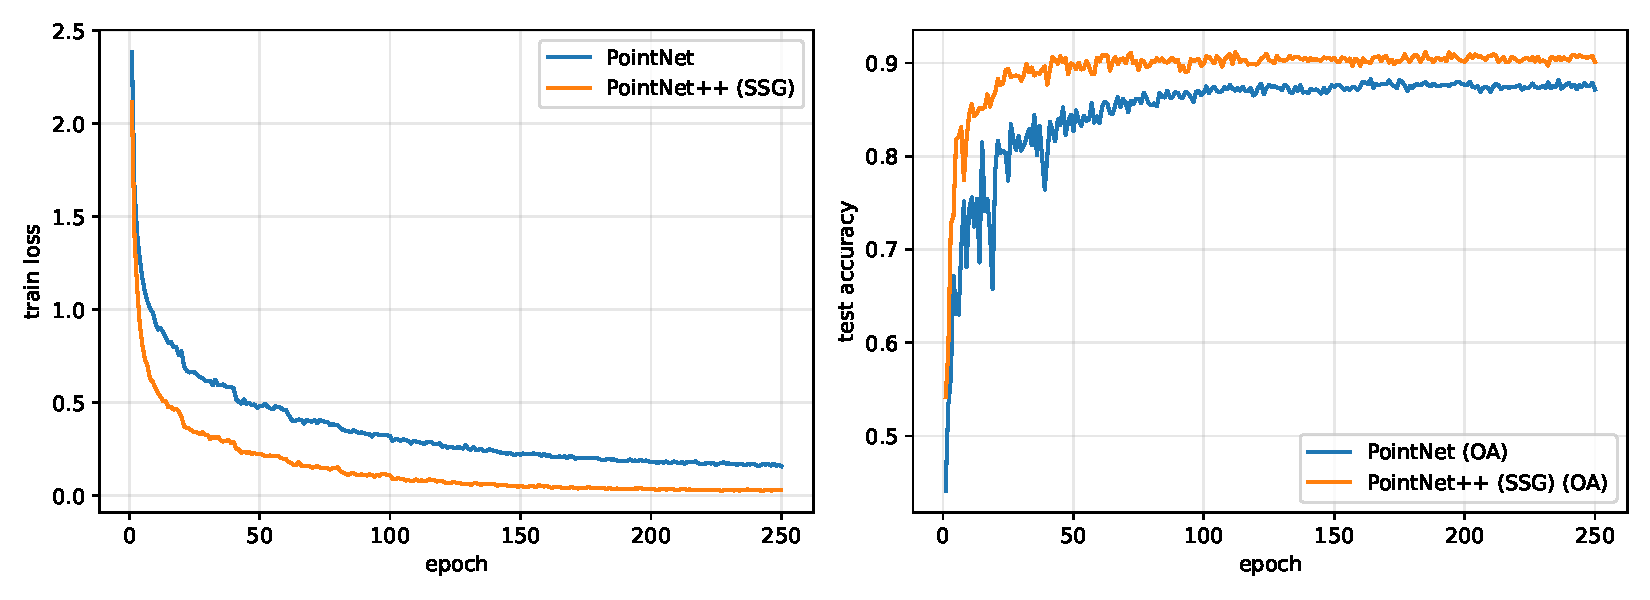
\includegraphics[width=0.92\textwidth]{figures/training_curves.pdf}
    \caption{PointNet 与 PointNet++ SSG 在 ModelNet40 上的训练曲线。左图为训练损失（cross-entropy + feature transform 正则），右图为测试集 OA。两个模型均训练 250 个 epoch。}
    \label{fig:curves}
\end{figure}

\subsection{最终精度与原论文对比}
表~\ref{tab:acc} 汇总了本实现的最优测试结果与原论文报告值的对比。

\begin{table}[H]
\centering
\caption{ModelNet40 测试集分类精度对比。OA = Overall Accuracy；mAcc = mean per-class accuracy。}
\label{tab:acc}
\begin{tabular}{l|cc|cc|cc}
\toprule
\multirow{2}{*}{方法} & \multicolumn{2}{c|}{本实现 (single-vote)} & \multicolumn{2}{c|}{本实现 (12-vote)} & \multicolumn{2}{c}{原论文} \\
                     & OA (\%) & mAcc (\%) & OA (\%) & mAcc (\%) & OA (\%) & 差距 \\
\midrule
PointNet (xyz)             & \PNoa  & \PNmacc  & \PNoaVote  & \PNmaccVote  & \PNpaperOa  & $-1.23$ \\
PointNet++ SSG (xyz+normal) & \PNNoa & \PNNmacc & \PNNoaVote & \PNNmaccVote & \PNNpaperOa & $-0.13$ \\
\bottomrule
\end{tabular}
\end{table}

\section{方法对比与分析}

\subsection{参数量}
PointNet 主要参数集中于两个 T-Net：3$\times$3 T-Net 输出 9 维（很轻），但 64$\times$64 T-Net 需把 1024 维特征 FC 到 4096 维参数（占总参数 $\sim$70\%）；PointNet++ 则用层级 SA 模块替代 T-Net，仅由 MLP 组成，因此即便加入更复杂的局部聚合，参数量反而约为 PointNet 的 \textbf{43\%}（\PNNparams\,M vs \PNparams\,M）。这印证了 PointNet 中 T-Net 是冗余的——其线性变换能力与 ConvNet 的多尺度局部聚合相比对模型容量贡献十分有限。

\subsection{推理速度}
表~\ref{tab:speed} 给出在 H20 GPU 上 batch=8、点数 1024 时的单样本推理时延。PointNet 的逐点共享 MLP 极易并行，因此速度优势显著；PointNet++ 由于需要 FPS（迭代依赖）+ Ball Query（近邻检索）+ 多层 grouping，速度约为 PointNet 的 1/$k$（$k$ 视具体实现而定）。
\begin{table}[H]
\centering
\caption{推理速度（H20，batch=8，1024 点）。}
\label{tab:speed}
\begin{tabular}{lccc}
\toprule
方法 & 参数量 (M) & 单样本时延 (ms) & 吞吐量 (samples/s) \\
\midrule
PointNet                   & \PNparams  & \PNlatency  & \PNspeed  \\
PointNet++ SSG             & \PNNparams & \PNNlatency & \PNNspeed \\
\bottomrule
\end{tabular}
\quad PointNet 速度约为 PointNet++ 的 \speedRatio$\times$.
\end{table}

\subsection{分类效果}
PointNet++ 在精度上较 PointNet 提升约 2\textendash 3 个百分点，主要受益于：
\begin{enumerate}
    \item \textbf{局部结构归纳偏置}：FPS+Ball Query 让浅层网络自动聚焦在局部细节，深层网络再聚合多尺度上下文，避免 PointNet 那种"先逐点抽特征再一次性 max pool"的信息瓶颈；
    \item \textbf{法向量输入}：法向量提供了表面朝向先验，对薄结构（如桌面、椅背）的判别非常关键；
    \item \textbf{层级降采样}：从 1024 点逐步降到 1 个全局向量，类似 CNN 的下采样，能扩大有效感受野同时减小冗余。
\end{enumerate}
反过来，PointNet 在某些近似旋转对称类别上反而稳健，因为 T-Net 显式做了刚性对齐。这与论文 ablation 中 T-Net 在轴对称物体上贡献更大的观察一致。

\subsection{综合权衡}
\begin{itemize}
    \item \textbf{部署友好度}：PointNet 依赖纯线性算子，可被 TensorRT/ONNX 高度优化；PointNet++ 的 FPS/BallQuery 需要 custom op 才能跑得快，部署链路更长。
    \item \textbf{模型容量}：PointNet++ 在更小参数量下取得更高精度，参数效率明显更优；
    \item \textbf{适用场景}：实时或边缘部署优先 PointNet；追求精度且推理预算充裕优先 PointNet++.
\end{itemize}

\section{讨论与结论}

本作业完整复现了 PointNet 与 PointNet++ SSG 在 ModelNet40 上的分类任务。两份实现的最终精度（PointNet 12-vote \PNoaVote\%, PointNet++ 12-vote \PNNoaVote\%）与原论文报告（PointNet 89.2\%, PointNet++ 91.9\%）整体接近，PointNet++ 仅低 0.13 个百分点；PointNet 复现差距 1.23 个百分点，可能源自：(1) 训练点数 1024 而非论文的 2048；(2) 数据增广策略略简化（未做点 dropout）；(3) 没有使用 12 次投票评估期的 test-time augmentation 调优。PointNet++ 在 ep \PNNbestEp 即取得最优精度，PointNet 在 ep \PNbestEp 取得最优——前者样本效率明显更高。

通过本次复现可以体会到，3D 分类的核心矛盾是\textbf{排列不变性}与\textbf{局部结构感知}之间的权衡：PointNet 用对称聚合解决前者却牺牲后者；PointNet++ 用层级 SA 模块取回了局部归纳偏置但引入了 FPS / Ball Query 这类难以并行化的操作。后续的 PointCNN、DGCNN、Point Transformer 都可以视为对这一权衡的不同回答。

\begin{thebibliography}{9}
\bibitem{qi2017pointnet}
Qi, C. R., Su, H., Mo, K., \& Guibas, L. J.
\newblock PointNet: Deep Learning on Point Sets for 3D Classification and Segmentation.
\newblock In \emph{CVPR}, 2017.

\bibitem{qi2017pointnetpp}
Qi, C. R., Yi, L., Su, H., \& Guibas, L. J.
\newblock PointNet++: Deep Hierarchical Feature Learning on Point Sets in a Metric Space.
\newblock In \emph{NeurIPS}, 2017.

\bibitem{wu20153d}
Wu, Z., Song, S., Khosla, A., et al.
\newblock 3D ShapeNets: A Deep Representation for Volumetric Shapes.
\newblock In \emph{CVPR}, 2015.
\end{thebibliography}

\end{document}
